\documentclass[12pt]{article}
\usepackage{amsmath}
\usepackage{listings}
\usepackage{textcomp}
\usepackage{graphicx}
\graphicspath{ {../images/} }

\usepackage[utf8]{inputenc} % allow utf-8 input
\usepackage[T1]{fontenc}    % use 8-bit T1 fonts
\usepackage{hyperref}       % hyperlinks
\usepackage{url}            % simple URL typesetting
\usepackage{booktabs}       % professional-quality tables
\usepackage{amsfonts}       % blackboard math symbols
\usepackage{nicefrac}       % compact symbols for 1/2, etc.
\usepackage{microtype}      % microtypography
\setlength{\parindent}{0pt}

\title{TITLE}

\author{
\begin{tabular}{ccc}
Ming~Cheng & Xingwei~Ji & Xiaofang~Jiang  \\
Fangzhou~Li & Diwen~Lu & Paul~Lu \\
Junyang~Shi & Jiayi~Xu & Timothy~Zhang \\
Haibin~Zhang & Feiwen~Zheng 
\end{tabular}
}

\begin{document}

\maketitle

\begin{abstract}
\quad We are doing prediction on result of National Collegiate Athletic Association (NCAA) Basketball game.  Before doing prediction, data will be processed to choose the most matching teams. Then we use model to predict on the result of next year for a regular season  using data of previous year. Two methods are applied for prediction. The first one is feeding preprocessed data into MPL. The second method is the application of logistic regression on the difference of features between two teams. 
\end{abstract}

\section{Introduction}

\quad to be finished

\section{Methods}

\quad To predict game results in 2018 by only knowing two team IDs playing against each other in each arranged game, there are 2 steps to be done. The first is to ascertain whether the team features we choose can best explain the game result. The second is to find a reliable approximation of team players post-game statistics for both old team players and new team players.

\subsection{Data Pre-processing}


\subsubsection{Generating post-game statistics for game results prediction}

\quad In finding which team post-game statistics can best explain the game results, we took data from RegularSeasonDetailedResults.csv, since we were only interested in the team as a whole and didn’t need to know post-game statistics for sepcific palyers. RegularSeasonDetailedResults.csv recorded game statistics (see TABLE1), as well as if it is a home, away, or neutral for winning team (“neutral” means the game is played in either of teams’ cities), and the day of game in that season. However, we don’t consider location and the day of match in our model. The reason is such information is outside inteference, and we expect it to have little influence on players’ performance. The file contains in total 76636 regular season gamses from 2003 to 2017. But among those years, we have playbyplay data only from 2010 to 2017, plus 2018, that have detailed records of each events that happend in each regular season game and each game’s players information. We decided to leave the game data from 2010 to 2017 for finding a reliable approximation of team players post-game statistics, and only use game results from 2003 to 2010 (39337 games) to check best team features to use in prediction model. For each team, there are 13 features (FGM, FGA, 3PM, 3PA, FTM, FTA, OR, DR, AST, TO, STL,BLK, PF) and 1 label (W/L) we took into consideration. And since we are not predicting concrete scores but the relative win and lose, we transferred 6 features each team that directly have influences on final score to 3 ratios (FG\%, 3P\%, FT\%) representing the shooting skill in field goal, three point, and free throw for each team, leaving only 10 features and 1 label now.

\quad Each line of \texttt{post\_game\_team\_diff.csv} is constructed as follows: \\


\lstset{language=Python, upquote=true}
\begin{lstlisting}[basicstyle=\small\tt]
For each game:
    for winning team
        for every i:
            feature_i_diff = Wteam_feature_i 
                           - Lteam_feature_i 
            W/L = 1 

    for losing team
        for every  i: 
            feature_i_diff = Lteam_feature_i 
                           - Wteam\_feature_i
            W/L = 0
\end{lstlisting}

\quad The reason is if we only take wining team as base team, then all labels would be 1, a very bad situation in which we have no instance of losing sample. At end, we have 78674 instances of games, half of them win instances and half lose instances.

\quad There are two problems with such representation. One is that the three shoorting percentages are of different magnitude from other team statistics. To ensure the computation precision and avoid error by cancellation, it is a bad habit to have data on different magnitudes. We multiple FG\%, 3P\%, and FT\% by 100 before taking difference between two teams and thus data are on the same scale now. The other issue is that some team didn’t even attempt ceratin type of shoot and divide 0 by 0 would yield NaN. There are only 36 instances (18 games) with NaN, tiny to our sample size at  , so we simply discarded these games from our samples. \\ 

The resulting data would look like: \\

(1st game in 2003)

\textbf{TABLE 1: 1st game in 2003 after rescale }

\begin{table}[h]
\begin{tabular}{llllllllll}
FG\%\_diff  & 3P\%\_diff & FT\%\_diff & OR\_diff & DR\_diff \\
0.504229018 & 1.42857143 & -11.616162 & 4  & 2 
\end{tabular} 
\end{table}

\begin{table}[h]
\begin{tabular}{llllllllll}
AST\_diff & TO\_diff & STL\_diff & BLK\_diff& PF\_diff\\
5 &5 &-1 &2 &1
\end{tabular} \\
\end{table}


\quad After generating team features differences for all games from 2003 to 2010, we wonder if there are any outliers that would affect bianry classification accuarcy. We performed isolation forest outlier detection on the dataset. The detector found total of 8839 outliers out of 78638 samples in the dataset. 

\subsubsection{Generating pre-game statistics for game result prediction}

\quad After having assured features we selected (FG\%\_diff, 3P\%\_diff, FT\%\_diff, OR\_diff, DR\_diff, AST\_diff, TO\_diff, STL\_diff, BLK\_diff, PF\_diff) strongly explain the game results (W/L), we moved on to find a way to estimate a team's post-game statistics before a game, and use the estimated team statistics to predict game result. We first calculates the ability scores in order to assign them to each player. Each player's ability scores are based on his performance in the last year. The scores are calculated by counting how many times a player performed each type of events. Since there are 21 different event types, we use 21 features to represent a player's ability information. Kaggle [3] provides event files, Events\_20XX.csv, recording each event conducted by a player with an ID and player files, Players\_20XX.csv, recording player IDs and player names. Player IDs started from 600001 to 642766 consecutively from 2010 to 2017. In order to reduce the accessing time, we read the player ID into a list, and to access the ability scores of player with the ID P, we could access by row index [P – 600001] of the list, which reducing O(n) searching problem into O(1).

\quad Then we calculates team features from 2011 to 2018 based on the performance of team players in the previous year. We need information about who played in which team. We assumed all team players would play in the game, and we obtained who they are by iterating each row in each Events\_20XX.csv and collected rows that belong to a single game and read player IDs that ever appeared in that game. A player might have multiple player IDs because he could show up in games in multiple years. For simplicity, we treated him as different players in different years, and we treated his first time appearance as a new player. Then we took the post-game statistics of each team players from the previous year, which represent our expectation of that player's performance in this year, and stored the whole team players post-game statistics in a data structure for later reference. For those new players in the team who never appeared in any games before, we took avg of all new players' post-game statistics from 2011 to 2017, and insert their information into that data structure, since we have no historical post-game statistics for this new players and this is the only way we can have a sense of how new players perform on average. For each game, we have expected post-game statistics for both teams and we calculate expected team post-game statistics based on its players data. 



\subsection{Model fitting}

\subsubsection{Multi-layer Perceptron}

\quad We first constructed a Multi-layer Perceptrons Python module with Tensorflow that allows a user to build an MLP binary classifier with user defined number of input features, hidden layers, neurons per hidden layer, and training epochs and other supporting features, such as performing parallel grid search on multiple CSIF machines,  plotting,  and saving weights, biases, and accuracies with both CSV and Tensorflow checkpoint format, to reduce computational time and the risk of data loss during training due to unexpected interruption. Only implementations are discussed here; details of instructions of running the module can be found in \texttt{/mlp/README.md}. \\

\textbf{Implementations of Layer Constructions}

\quad The implementation of building an MLP with user defined number of input features, hidden layers, and neurons per hidden layers is divided into three parts: Building the first hidden layer, building the output layer, and building the other hidden layers. In most Neural Network implementation, including Tensorflow, the weights and biases of each layer are stored in matrice. Since our module uses Tensorflow, this implies that the matrice of the weights of the first hidden layer, output layer, and other hidden layers in between have the dimensions of $F \times N$, $N \times 1$, and $N \times N$ respectively, where $F$ is the number of features and $N$ is the number of nodes in each hidden layer. Similarly, the dimensions of the bias matrice of the output layer and other layers are $1 \times 1$ and $1 \times N$ respectively.  Now that we have matrice of weights and biases of all layers, the only thing left to do is to connect them together. We do this by connecting the first hidden layer to the input placeholders and the rest to their previous layers with each layer's sigmoid activation function as shown below.  

\begin{align}
f(z) &= \dfrac{1}{1+e^z}  \\
a^{(1)} &= f(X \times W^{(1)} + b^{(1)}) \\
a^{(2)} &= f(a^{(1)} \times W^{(2)} + b^{(2)})\\
... \\
a^{(L)} &= f(a^{(L-1)} \times W^{(L)} + b^{(L)})\\
a^{(out)} &= f(a^{(L)} \times W^{(out)} + b^{(out)})
\end{align}

where $L$ is the number of hidden layers. \\ 


\textbf{Implementation of Progress Saving \& Plotting}

\quad The implementation of saving progress is done in two different ways. One way is saving all variables and the Tensorflow graph with Tensorflow checkpoint format. The other way is through saving the accuracies of both training and testing and values of the matrices of weights and biases of each epoch in a CSV file. The former is used for resuming progress to avoid progress loss, and the latter is mainly for logging and plotting. There are also two types of CSV file that can be chosen to save the weights, and they are called "compact" and "detailed." A compact CSV file is for plotting a "compact plot" which consists of the change of the mean weight of each layer through iterations, and a detailed CSV file is for plotting a "detailed plot" which contains the change of every individual weight of each layer through iterations. Due to the large number of input features, using a detailed plot is not recommended since the mean weights of a layer is already capable of showing the convergence of that layer and is much clearer in plots. Users also have the option to save a detailed CSV file with every individual weight and graph a compact plot from this CSV afterwards. \\ 


\textbf{Implementation of Parallel Grid Search with CSIF}

\quad The implementation of grid search is done in a function that invokes different sessions of terminals that send commands to user chosen CSIF machines through SSH which have individual CSIF machines to build and train individual MLP with number of neurons and layers defined within user defined range. The accuracies from each model are printed back to each terminal and other results, such as CSV files and Tensorflow checkpoint files are saved on the CSIF machines under user's account. This parallel implementation of grid search with multiple CSIF machines dramatically reduce the computational time and also allow users' local machines to perform other tasks. \\

\textbf{Implementation of Testing Functions} 

\quad We have also included testing datasets and their generator in \texttt{mlp/fake\_\\feature}. All datasets have 10 columns of input features and 1 column of binary outputs. The input features are generated with normal distribution with slightly different mean and standard deviations. The binary output of each row is based on the value of $f$ below

\begin{align}
f &= 0.5*(a_f1-b_f1) + 0.3*(a_f2-b_f2) - 0.6*(a_f3-b_f3) \\
   &+ 0.4*(a_f4-b_f4) - 0.4*(a_f5-b_f5)\\
   &+ [\text{a random number uniformly picked between -250 $\sim$ 250 as noise}]
\end{align}

and the output is 1 if $f$ is greater than one and 0 otherwise. The main testing dataset \texttt{mlp/fake\_feature/feature.csv} has $10,000$ rows and was fed into the MLP that we have built. The model successfully fits the simple dataset almost instantaneously. As expected, the accuracies of the model were limited by the noise created and reached $99.21\%$ when the noise was removed. \\


\textbf{Running on Post-Game Data}

\quad After confirming that our MLP module functions correctly, we fed the post-game data into our model and started to train. To feed, train, and teston the post-game dataset, we can just use the following command

\lstset{language=Python, upquote=true}
\begin{lstlisting}[basicstyle=\small, numbers=left]
from mlp.mlp import *
m=Mlp(
    'post_game', n_feat=10, n_hidden=0, n_node=1, 
     n_epoch=50, n_train=55048,
     pathToDataset='./data_processing/output/'
                   'post_game_team_diff.csv',
     random=True, seed=1234, compact_plot=False,
     intvl_save=5, intvl_write=1, intvl_print=1,
     normalization='nor')
m.new_model()
m.train_model(0)
\end{lstlisting}

\textbf{Running on Pre-game data}

\quad For pre-game data, we uploaded our directory to CSIF and started a grid search on the data for 0 to 3 hidden layers and 1 to 6 neurons for 100 epochs with the following command (Note: to use the following function, user must set up keyless login\footnote{CSIF keyless login setup: \\ http://csifdocs.cs.ucdavis.edu/about-us/csif-general-faq\#TOC-How-do-I-set-up-SSH-keys-to-allow-me-to-login-to-the-CSIF-computers-without-a-password-} and assure that the machines to be used are not down\footnote{CSIF status: \\ http://iceman.cs.ucdavis.edu/nagios3/cgi-bin/status.cgi?hostgroup=all}. More details on running the function, including the argument descriptions, are inside of the function description in \texttt{/mlp/mlp.py}): 

\lstset{language=Python, upquote=true}
\begin{lstlisting}[basicstyle=\small, numbers=left]
from mlp.mlp import *
import os

pc = ['1', '2', '3', '4', '5', '6', '7', '8', '9', '10',
     '11', '12', '13', '14', '15', '16', '17', '18', '19']
parallel_csif_grid_search(
   'mtimzh', pc, '/home/mtimzh/ECS-171-Group-Project',
   'NCAA', 42, 100, 40113,
   './pre_game_teams', intvl_save=2000, r_l=0.1,
   intvl_write=1, intvl_print=1, compact_plot=False,
   max_to_keep=1, n_grid_layer=4, n_grid_neuron=6
   )
\end{lstlisting}

\quad The first 40113 rows of the dataset was chosen as the training set because the row of the first match in 2018 starts at 40114, and we are trying to make predictions on the matches in 2018, After all of the trainings have finished, we can download all of the CSV output files to our local machine from \texttt{/mlp/datapoints/} on the CSIF machines  (although we are running multiple CSIF machines, everything is stored in the same directory due to CSIF's file system)  and plot them with 

\lstset{language=Python, upquote=true}
\begin{lstlisting}[basicstyle=\small, numbers=left]
# Assume we have downloaded the CSV files to the path below
rootdir = './mlp/datapoints/'
for dir, subdirs, fs in os.walk(rootdir):
   for f in fs:
       plot_compact_from_detailed(os.path.join(dir,f))
\end{lstlisting}


\subsubsection{Logistic Regression}

\textbf{Implementation}

\quad This is a simple implementation with the \texttt{glm} function in \texttt{R}. We simply first split the dataset into training and testing, compute the weights with the \texttt{glm} function by feeding in the training set, and calculate the accuracies by using the \texttt{predict} function. \\

\textbf{Running on Post-Game and Pre-Game Data}
To run on the post-game data, we can just pass the following command into terminal:
\lstset{upquote=true}
\begin{lstlisting}[basicstyle=\small, numbers=left]
rscript logitReg/logitReg.R 
\end{lstlisting}

\section{Results}
\subsection{Results on post-game statistics game results prediction}
\quad We wanted to visualize multi-dimensional data in post-game statistics in outlier detection by t-SNE, and the algorithm reduced multi-dimensional data to only 2 dimensions to better illustrate the distribution of the data. However, we saw no outstanding outliers in the reduced 2 dimensional t-SNE plot. And by comparing the result between before removing outliers and after removing outliers, we saw no significant improvement on testing accuracy, which further supported our claim that post-game statistics for all teams are very close to each other. We actually reached a higher testing accuracy without removing outliers. \\

\textbf{T-NSE}

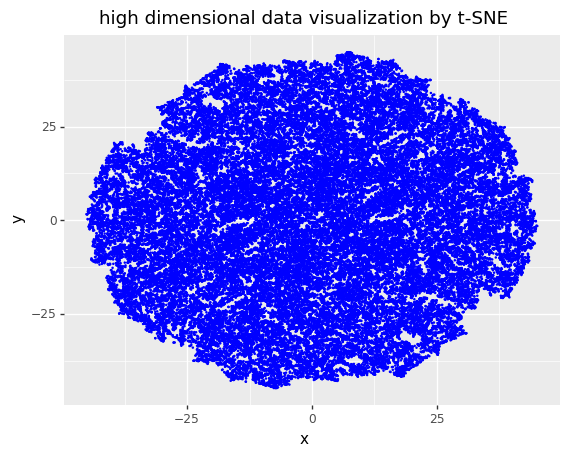
\includegraphics[scale=0.9]{tsne.png} 

\textbf{Outlier detection in data-processing for post-game statistics for game results}

\quad After deciding not doing outlier detection, we tried MLP with several different number of hidden layers and number of hidden neurons but they all converged to same testing accuracy very quickly. Then we tried logistic regression in R and found it showed around same testing accuracy as was in MLP model. We decided to use MLP in pre-game statistics for game result prediction since it is more versatile. \\ 

\textbf{Mean Weight vs Epoch\qquad \qquad Accuracy vs Epoch} \\
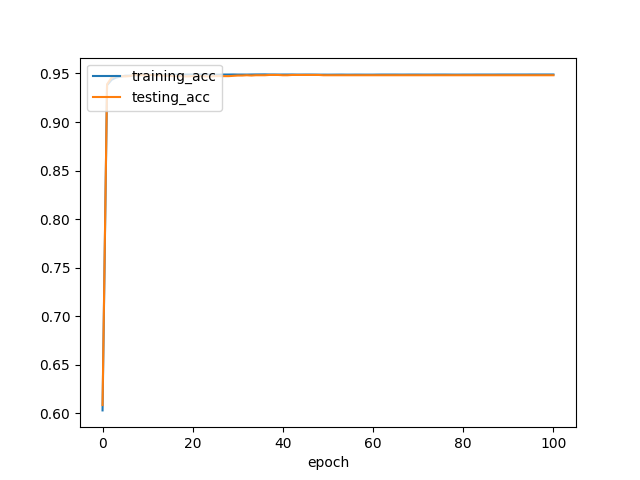
\includegraphics[scale=0.4]{postGame_0_1_compact_accuracy.png} 
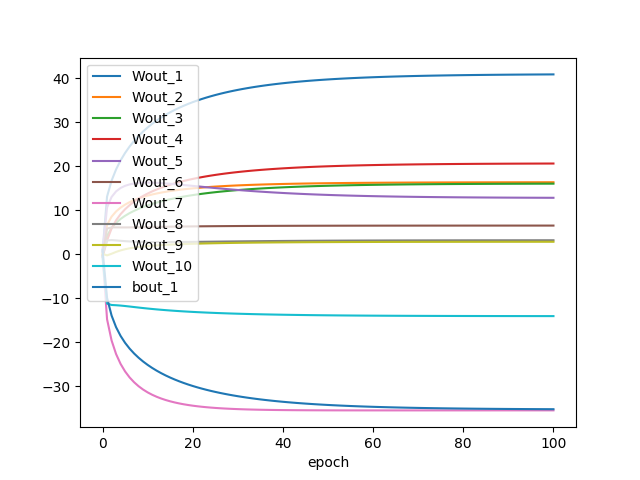
\includegraphics[scale=0.4]{postGame_0_1_detailed_weights.png} 

\textbf{TABLE 3: 10 weights of 10 features in post-game statistics MLP game result prediction }

\begin{table}[h]
\begin{tabular}{llllllllll}
FG\%\_diff & 3P\%\_diff & FT\%\_diff  & OR\_diff   & DR\_diff \\
40.828392  & 16.331735  & 16.0064106  & 20.5814533 & 12.79597 
\end{tabular}
\end{table}

\begin{table}[h]
\begin{tabular}{llllllllll}
AST\_diff &TO\_diff & STL\_diff & BLK\_diff& PF\_diff\\
6.48547268  &-35.493058 & 3.15093279 & 2.80670953 & -14.080395
\end{tabular}
\end{table}

Interestingly, we notice only 2 features have negative weights, and they are TO\_diff and PF\_diff. It makes sense because turnovers and persona fouls has an negative impacting on a team's scoring and would let the opponent team score more.

\subsection{Results on pre-game statistics game results prediction}
\quad Combined versions of the MLP plots on pre-game data\footnote{Individual images can be found in \texttt{/mlp/NCAA\_preGame/plots/}.} for grid search on [1, 6] layer neuron and [1, 3] hidden layers are on the next two pages, where row number is the number of neurons per layer, and column number is the number of hidden layer. The plots for grid search on no hidden layer are on the page after. \newpage

\textbf{Mean Weights vs Epoch}

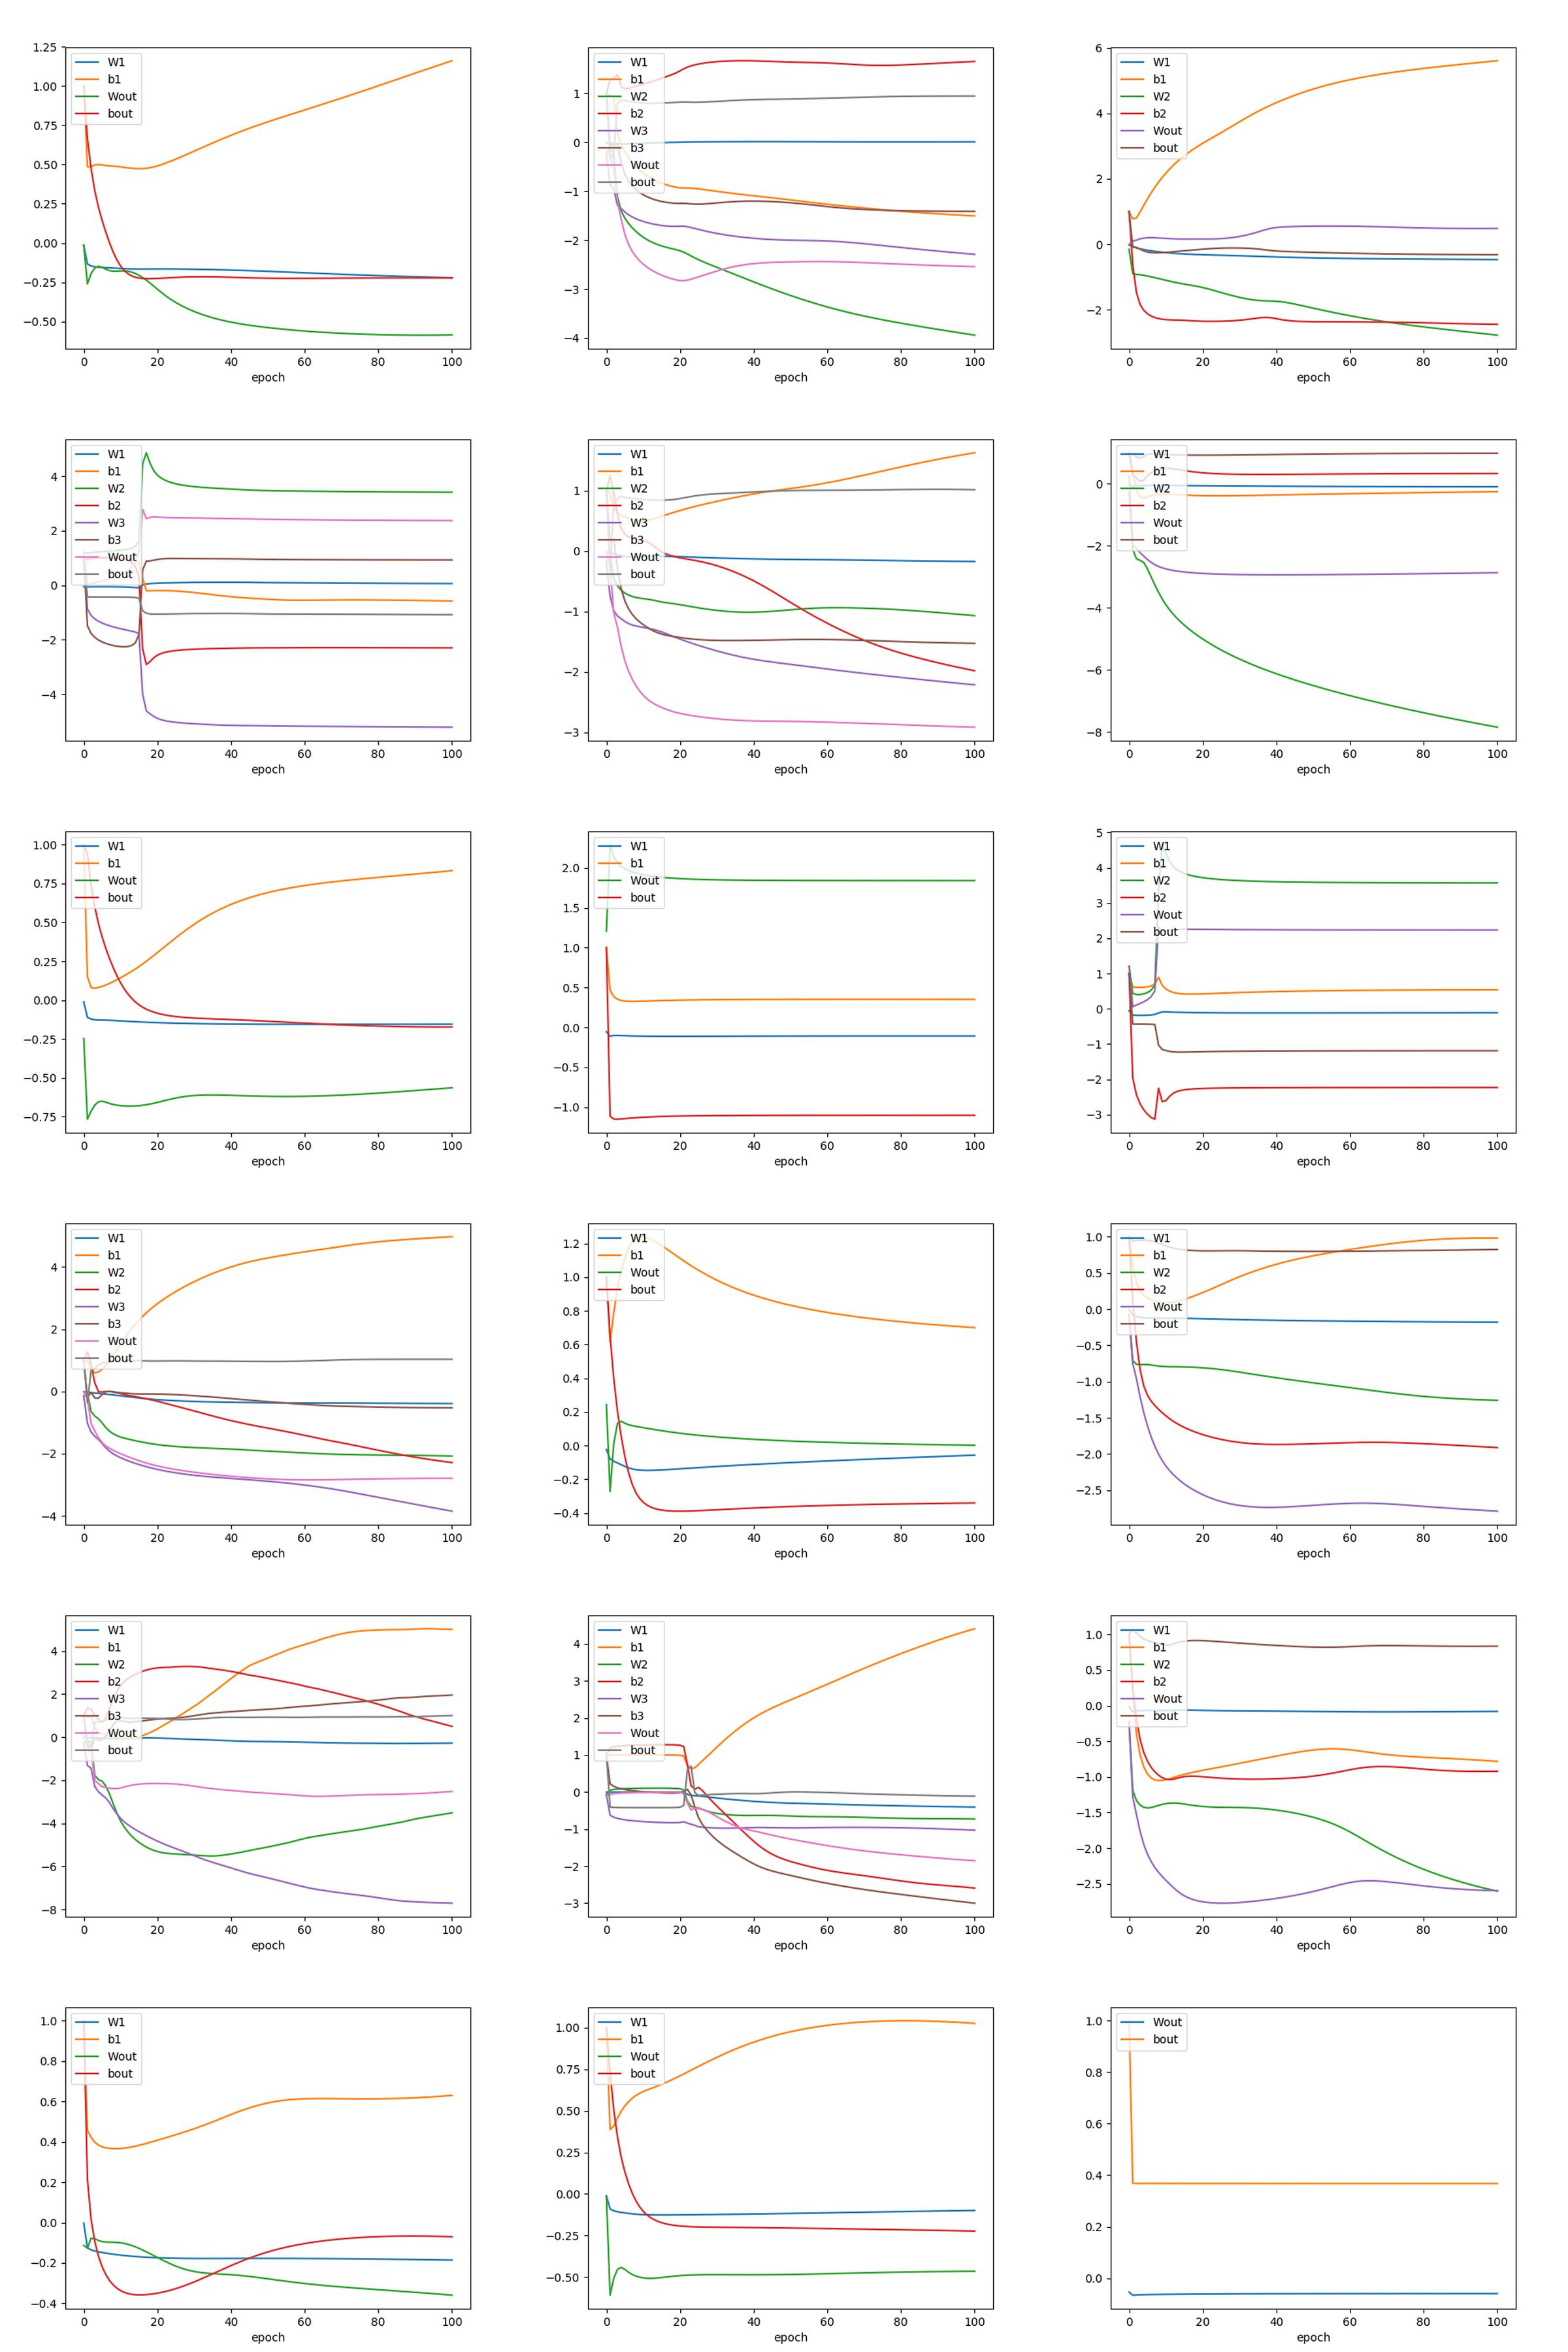
\includegraphics[scale=0.145]{NCAA_18_weights.jpg} \newpage 

\textbf{Accuracy vs Epoch}

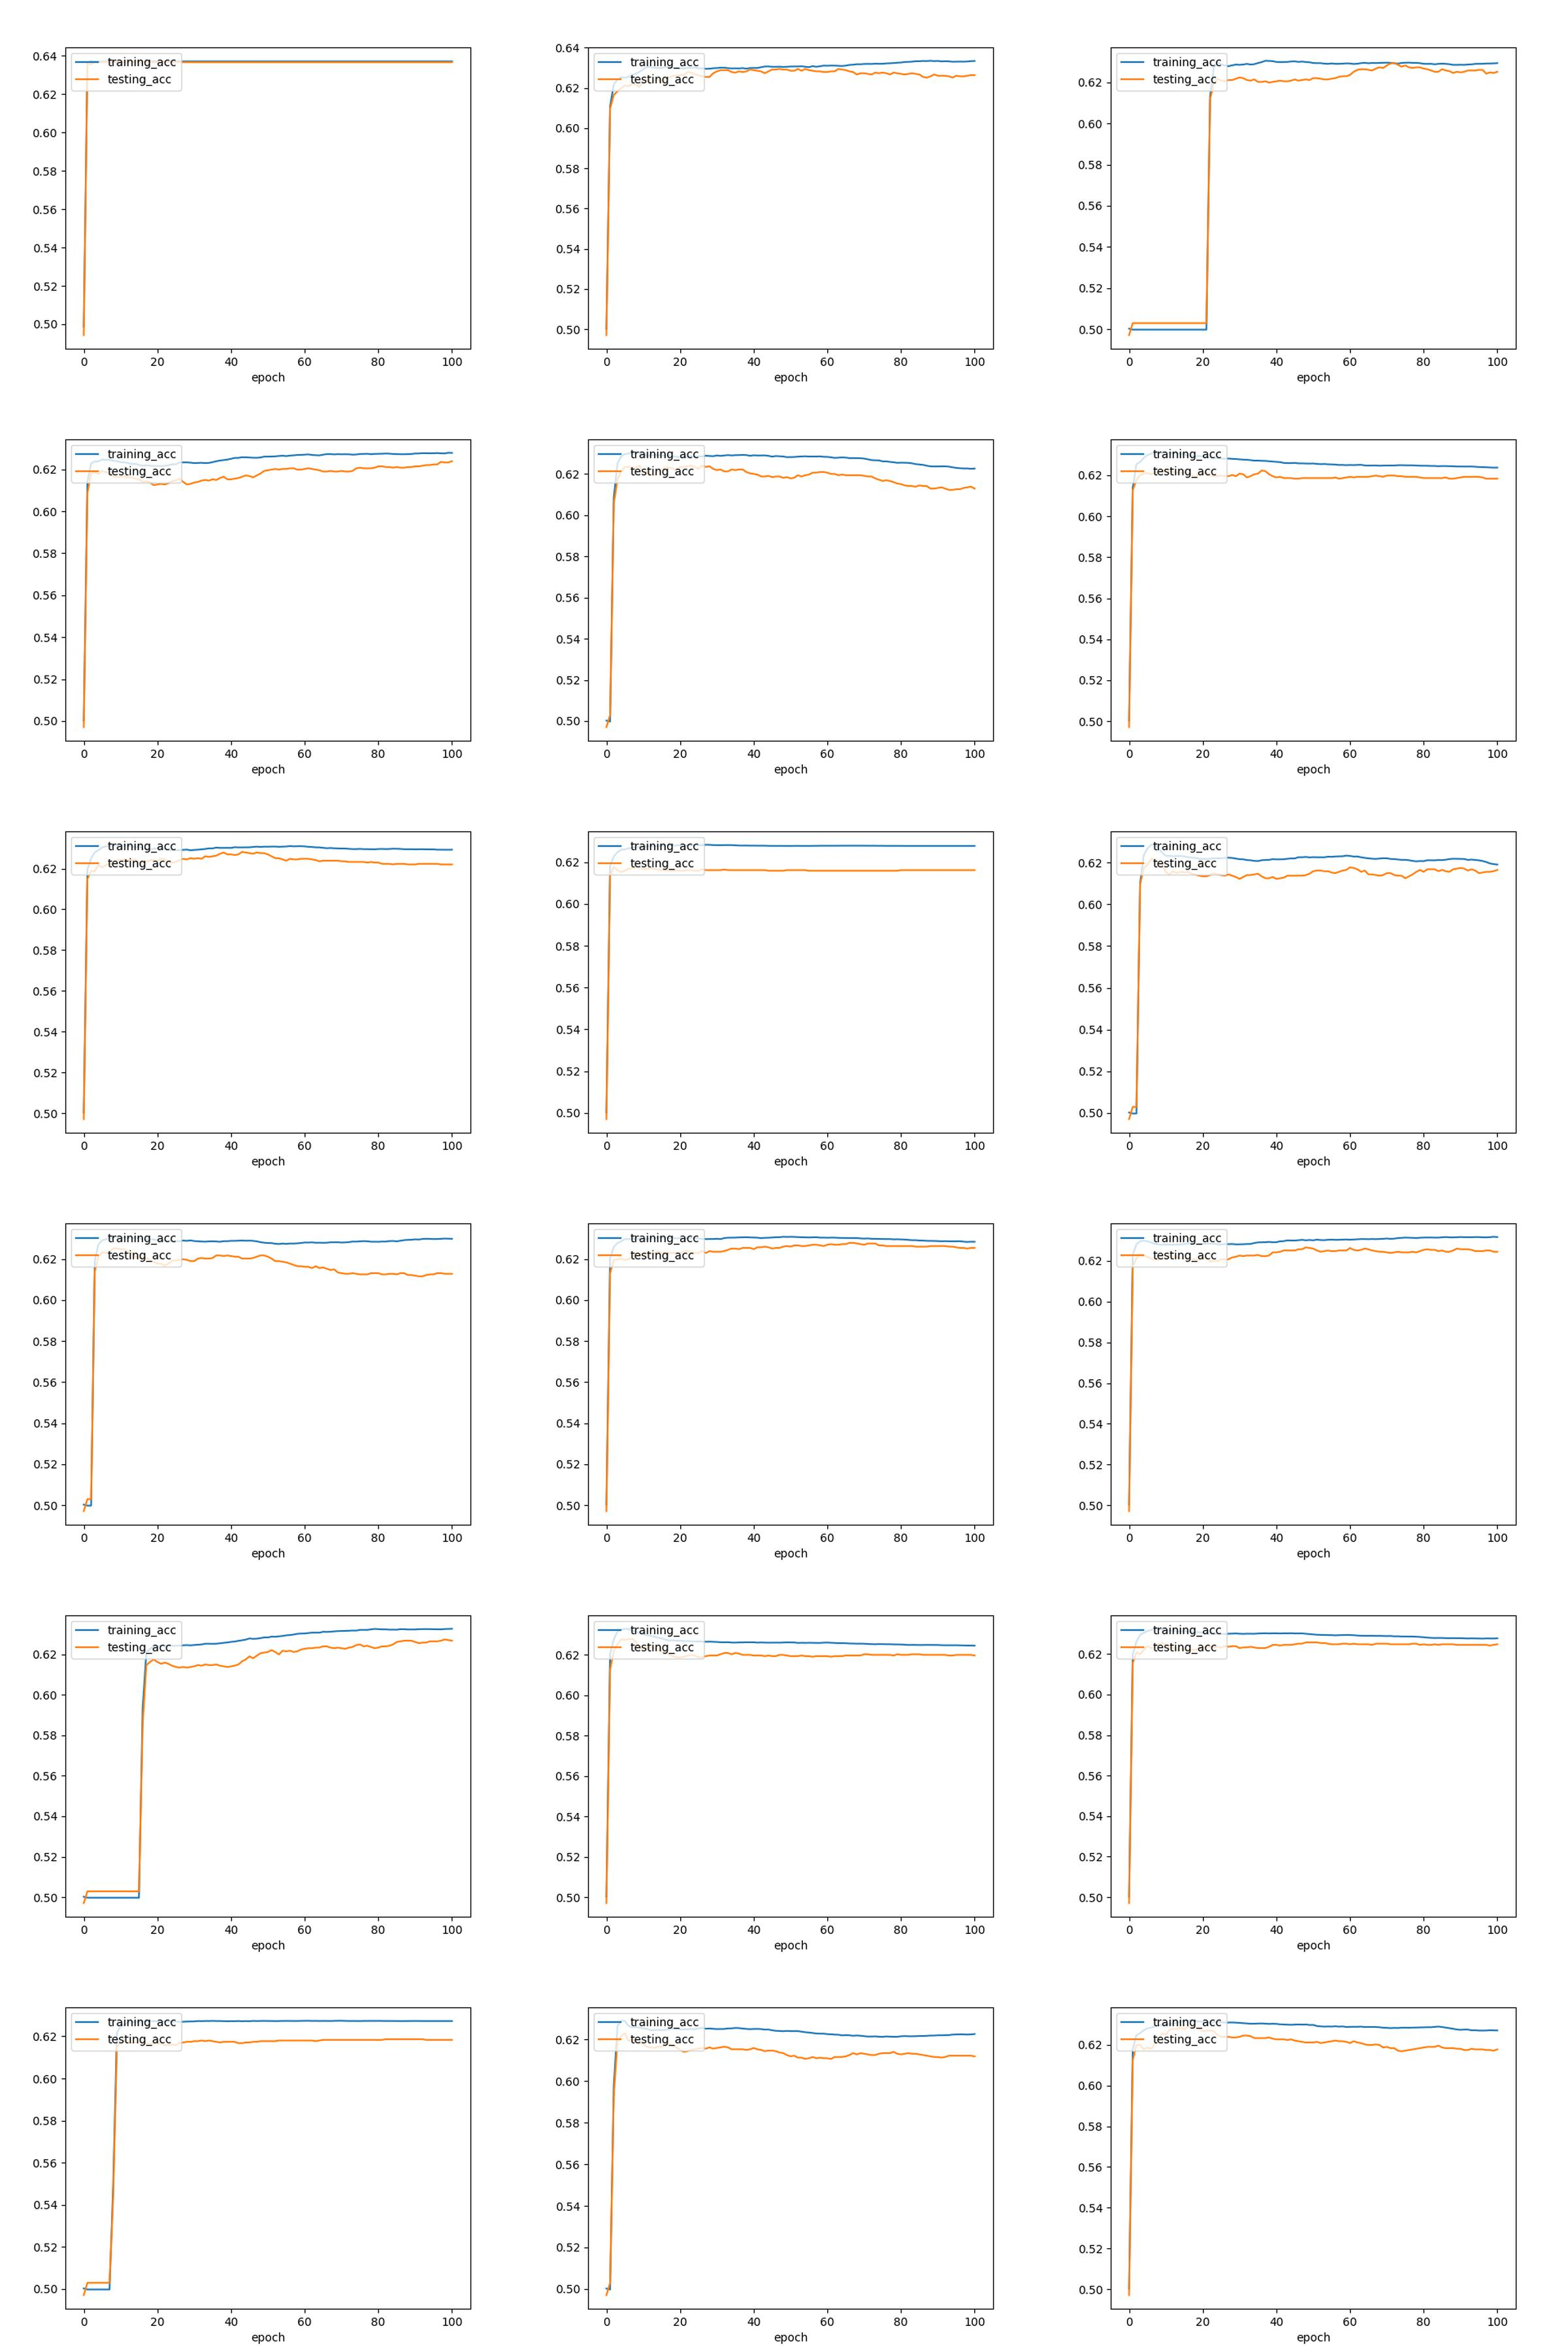
\includegraphics[scale=0.145]{NCAA_18_accuracy.jpg} \newpage

\textbf{Mean Weight vs Epoch\qquad \qquad Accuracy vs Epoch}

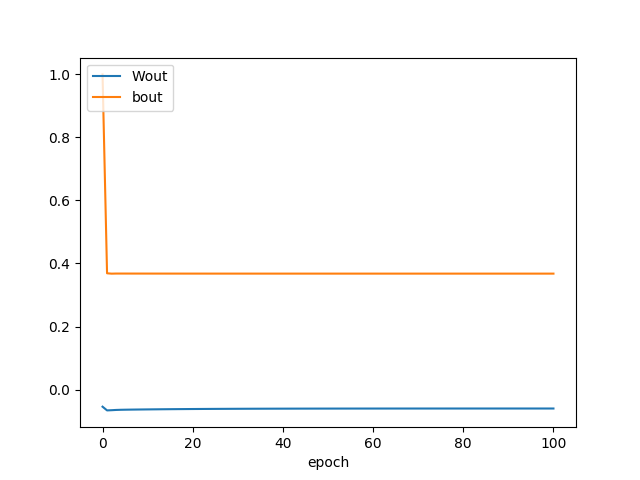
\includegraphics[scale=0.4]{NCAA_0_1_compact_weights.png} 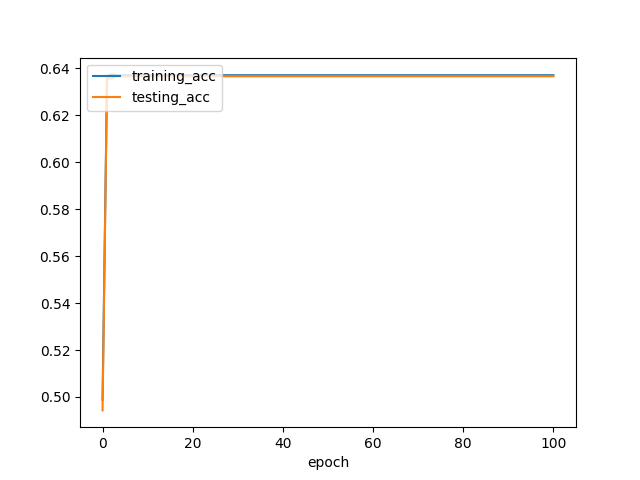
\includegraphics[scale=0.4]{NCAA_0_1_compact_accuracy.png} \\ 


\quad Results from running the logistic regression model are shown below:


\lstset{upquote=true}
\begin{lstlisting}[basicstyle=\small, numbers=left]
$ rscript logitReg/logitReg.R 
Running ./data_processing/output/post_game_team_diff.csv
Training Accuracy:	0.9488
Testing Accuracy:	0.9489
Running ./pre_game_teams.csv
Training Accuracy:	0.647
Testing Accuracy:	0.6032
\end{lstlisting}



\section{Discussion}



\section*{References (Samples)}
\qquad \qquad \qquad \qquad \qquad \qquad \qquad \qquad \qquad \qquad \qquad \qquad \qquad \qquad \qquad \qquad \qquad \qquad \qquad \qquad \qquad \qquad \qquad \qquad \qquad \qquad .
 
\small
[1] Alexander, J.A.\ \& Mozer, M.C.\ (1995) Template-based algorithms for
connectionist rule extraction. In G.\ Tesauro, D.S.\ Touretzky and T.K.\ Leen
(eds.), {\it Advances in Neural Information Processing Systems 7},
pp.\ 609--616. Cambridge, MA: MIT Press.

[2] Bower, J.M.\ \& Beeman, D.\ (1995) {\it The Book of GENESIS: Exploring
  Realistic Neural Models with the GEneral NEural SImulation System.}  New York:
TELOS/Springer--Verlag.

[3] Hasselmo, M.E., Schnell, E.\ \& Barkai, E.\ (1995) Dynamics of learning and
recall at excitatory recurrent synapses and cholinergic modulation in rat
hippocampal region CA3. {\it Journal of Neuroscience} {\bf 15}(7):5249-5262.

\end{document}
